\documentclass[12pt]{article}
\pdfoutput=1

\newcommand{\VersionInformation}{}  % overwritten by Debug.tex
\InputIfFileExists{Debug}{}{}


\usepackage[utf8]{inputenc}
\usepackage{amsmath}
\usepackage{amsthm}
\usepackage{amsfonts}          % if you want the fonts
\usepackage{amssymb}           % if you want extra symbols
%\usepackage{euscript}
\usepackage[mathscr]{eucal}
%\usepackage{stmaryrd}          % \lightning is defined there
\usepackage{graphicx}
\usepackage{color}
%\usepackage{floatflt}
%\usepackage{bbold}
%\usepackage{ulem}
\usepackage[nosort]{cite}
\usepackage{hypbmsec}
\usepackage{fancyvrb}
\usepackage{sepnum}
\usepackage{xspace}
\usepackage{booktabs}
\usepackage{rotating}
\usepackage{multirow}
\usepackage[vcentermath]{youngtab}
%\usepackage{slashbox}
\usepackage{simplewick}
\usepackage[isu,bf]{caption}
\setlength{\captionmargin}{1cm}
\renewcommand{\captionfont}{\small\itshape}


%\usepackage{algorithm}
%\usepackage{algorithmic}

\font\csc=cmcsc10

\newlength{\xtrawidth}
\setlength{\xtrawidth}{8mm}
\newlength{\xtraheight}
\setlength{\xtraheight}{10mm}
\addtolength{\textwidth}{\xtrawidth}
\addtolength{\textwidth}{\xtrawidth}
\addtolength{\oddsidemargin}{-\xtrawidth}
\addtolength{\evensidemargin}{-\xtrawidth}
\addtolength{\textheight}{\xtraheight}
\addtolength{\textheight}{\xtraheight}
\addtolength{\topmargin}{-\xtraheight}


\usepackage[all]{xy}           % Commutative diagrams



\ifx\NoBackreferences\EMPTYMACRO
  % arXiv will complain about option clash in hyperref
  % \usepackage[backref,linktocpage,bookmarks]{hyperref}
  \usepackage{hyperref}
\else
  \usepackage[linktocpage,bookmarks]{hyperref}
\fi

% \usepackage[sort&compress]{natbib}


\def\footnoteautorefname{Footnote}%
\def\itemautorefname{Item}%
\def\sectionautorefname{Section}%
\def\subsectionautorefname{Subsection}%
\def\subsubsectionautorefname{Subsubsection}%
\def\paragraphautorefname{Paragraph}%
\def\subparagraphautorefname{Subparagraph}%
\def\FancyVerbLineautorefname{Line}%

%%%%%%%%%%%%%%% volker's defs %%%%%%%%%%%%%%%

% \entrymodifiers={[F.]}
%\usepackage[floats,textmath,displaymath,delayed,sections,auctex]{preview}

\ifx\DEBUG\EMPTYMACRO
  % Don't use showlabels
\else
  \usepackage{showlabels}
\fi


\newcommand{\lrstack}[3][t]{
  \ensuremath{
    \begin{array}[#1]{c}
      \multicolumn{1}{l}{\displaystyle{#2}\quad} \\[0.5em] 
      \multicolumn{1}{r}{\displaystyle\quad{#3}}
    \end{array}
  }}
\def\clap#1{\hbox to 0pt{\hss#1\hss}}
\def\mathllap{\mathpalette\mathllapinternal}
\def\mathrlap{\mathpalette\mathrlapinternal}
\def\mathclap{\mathpalette\mathclapinternal}
\def\mathllapinternal#1#2{%
\llap{$\mathsurround=0pt#1{#2}$}}
\def\mathrlapinternal#1#2{%
\rlap{$\mathsurround=0pt#1{#2}$}}
\def\mathclapinternal#1#2{%
\clap{$\mathsurround=0pt#1{#2}$}}	

\makeatletter
  \def\adots{\mathinner{\mkern2mu\raise\p@\hbox{.}
      \mkern2mu\raise4\p@\hbox{.}\mkern1mu
      \raise7\p@\vbox{\kern7\p@\hbox{.}}\mkern1mu}}
\makeatother

\newcommand{\comma}[1]{\ensuremath{\sepnum{{.}}{{,}}{}{#1}}}


\newcommand{\eqdef}{%
  \mathrel{\lower.1mm
    \hbox{$\stackrel{\lower.424ex\hbox{\scriptsize def}}{=}$}}
}
%\newcommand{\eqdef}{\stackrel{\mathrm{def}}{=}}
%\newcommand{\eqdef}{=}
\newcommand{\Q}{\ensuremath{{\mathbb{Q}}}}
\newcommand{\R}{\ensuremath{{\mathbb{R}}}}
\newcommand{\C}{\ensuremath{{\mathbb{C}}}}
\newcommand{\Hbb}{\ensuremath{{\mathbb{H}}}}
\newcommand{\Z}{\mathbb{Z}}
% \newcommand{\CP}{\ensuremath{\mathop{\mathbb{C}{\rm P}}}\nolimits}
\newcommand{\CP}{{\ensuremath{\mathop{\null {\mathbb{P}}}\nolimits}}}
\newcommand{\IP}{{\ensuremath{\mathop{\null {\mathbb{P}}}\nolimits}}}
\newcommand{\RP}{\ensuremath{\mathop{\mathbb{R}{\rm P}}}\nolimits}
\newcommand{\F}{\ensuremath{{\mathbb{F}}}}

\newcommand{\ibar}{\ensuremath{{\bar{\text{\it\i\/}}}}}
\newcommand{\jbar}{\ensuremath{{\bar{\text{\it\j\/}}}}}
\newcommand{\alphabar}{\ensuremath{{\bar{\alpha}}}}
\newcommand{\betabar}{\ensuremath{{\bar{\beta}}}}
\newcommand{\sbar}{\ensuremath{{\bar{s}}}}
\newcommand{\zbar}{\ensuremath{{\bar{z}}}}

\newcommand{\FS}{\ensuremath{{\text{FS}}}}

\newcommand{\Dbrane}{D-brane}
\newcommand{\Dbranes}{D-branes}
\newcommand{\YM}{Yang-Mills}
\newcommand{\MW}{Mordell-Weil}
\newcommand{\MWgrp}{\MW{} group}
\newcommand{\MWlat}{\MW{} lattice}
\newcommand{\even}{\ensuremath{\mathrm{ev}}}
\newcommand{\odd}{\ensuremath{\mathrm{odd}}}
\newcommand{\Ktheory}{K-theory}
\newcommand{\Ktheories}{K-theories}
\newcommand{\Kgroup}{K-group}
\newcommand{\Kgroups}{K-groups}
\newcommand{\KRtheory}{KR-theory}
\newcommand{\KRtheories}{KR-theories}
\newcommand{\KRgroup}{KR-group}
\newcommand{\KRgroups}{KR-groups}
\newcommand{\KOtheory}{KO-theory}
\newcommand{\Ktilde}{\widetilde{K}}
\newcommand{\KOtilde}{\widetilde{KO}}
\newcommand{\Kan}{K_\mathrm{an}}
\newcommand{\Kcoh}{K_\mathrm{coh}}
\newcommand{\Kalg}{K_\mathrm{alg}}
\newcommand{\Cech}{{\v{C}ech}}
\newcommand{\Hcech}{{\check{H}}}
\newcommand{\Hdr}{H_\mathrm{DR}}
\newcommand{\Hol}{\mathrm{Hol}}
\newcommand{\Kunneth}{K{\"u}nneth}
\newcommand{\inv}{\mathrm{inv}}

\newcommand{\Ncal}{\mathcal{N}}
\newcommand{\tKop}[1]{\ensuremath{\vphantom{K}^{#1}\!K}}
\newcommand{\tK}{\ensuremath{\tKop{t}}}
\newcommand{\T}[1]{\lbrack{#1}\rbrack} % shift functor X[i]
\newcommand{\ptset}{\ensuremath{\{\text{pt.}\}}}
\newcommand{\iunit}{\ensuremath{\mathrm{i}}}
\newcommand{\Cunits}{\ensuremath{\C^\times}}
\newcommand{\free}{\ensuremath{\text{free}}}
\newcommand{\tors}{\ensuremath{\text{tors}}}

\newcommand{\Moduli}{\mathcal{M}}
\newcommand{\rt}{\ensuremath{\tilde{r}}}

\DeclareMathOperator{\Div}{Div}
\DeclareMathOperator{\TDiv}{TDiv}


\DeclareMathOperator{\diff}{d\!}
\DeclareMathOperator{\Span}{span}
\DeclareMathOperator{\Pic}{Pic}
\DeclareMathOperator{\re}{re}
\DeclareMathOperator{\im}{im}
\DeclareMathOperator{\Tr}{Tr}
\DeclareMathOperator{\tr}{tr}
\DeclareMathOperator{\Mat}{Mat}
\DeclareMathOperator{\Id}{id}
\DeclareMathOperator{\rank}{rank}
\DeclareMathOperator{\codim}{codim}
\DeclareMathOperator{\End}{End}
\DeclareMathOperator{\Aut}{Aut}
\DeclareMathOperator{\Sym}{Sym}
\DeclareMathOperator{\Alt}{Alt}
\DeclareMathOperator{\idx}{Index}
\DeclareMathOperator{\img}{img}
\DeclareMathOperator{\coker}{coker}

\DeclareMathOperator{\Hom}{Hom}
\DeclareMathOperator{\Tor}{Tor}
\DeclareMathOperator{\Ext}{Ext}

\DeclareMathOperator{\HOM}{\underline{Hom}}
\DeclareMathOperator{\TOR}{\underline{Tor}}
\DeclareMathOperator{\EXT}{\underline{Ext}}

\DeclareMathOperator{\Sing}{Sing}
\DeclareMathOperator{\Li}{Li}
\DeclareMathOperator{\Vol}{Vol}
\DeclareMathOperator{\dVol}{dVol}
\DeclareMathOperator{\diag}{diag}

\DeclareMathOperator{\Ind}{Ind}
\DeclareMathOperator{\Res}{Res}
\DeclareMathOperator{\AltInd}{AltInd}
\DeclareMathOperator{\SymInd}{SymInd}
\DeclareMathOperator{\GrInd}{GrInd}

\DeclareMathOperator{\Stab}{Stab}

\newcommand{\Spin}{{\mathop{\text{\textit{Spin}}}\nolimits}}
\newcommand{\sofrak}{{\mathop{\mathfrak{so}}\nolimits}}
\newcommand{\sufrak}{{\mathop{\mathfrak{su}}\nolimits}}
\newcommand{\hfrak}{{\mathop{\mathfrak{h}}\nolimits}}
\newcommand{\soTenC}{{\mathop{\sofrak(10)_\C}\nolimits}}
\newcommand{\Rep}[1]{\ensuremath{\mathbf{\underline{#1}}}}
\newcommand{\barRep}[1]{\ensuremath{\overline{\Rep{#1}}}}
\DeclareMathOperator{\Reg}{Reg}
\DeclareMathOperator{\Ad}{ad}


\newcommand{\textdef}[1]{\textit{#1}}

\newcommand{\Xt}{{\ensuremath{\widetilde{X}}}}
\newcommand{\Vt}{{\ensuremath{\widetilde{V}}}}
\newcommand{\Xb}{{\ensuremath{\overline{X}}}}
\newcommand{\Ct}{{\ensuremath{\widetilde{C}}}}
\newcommand{\ZZZ}{\ensuremath{{\Z_3\times\Z_3}}}
\newcommand{\Lsheaf}{\ensuremath{\mathscr{L}}}
\newcommand{\Osheaf}{\ensuremath{\mathscr{O}}}
\newcommand{\OsheafXt}{\ensuremath{\mathscr{O}_{\Xt}}}
\newcommand{\OsheafBone}{\ensuremath{\mathscr{O}_{B_1}}}
\newcommand{\OsheafBtwo}{\ensuremath{\mathscr{O}_{B_2}}}
\newcommand{\OsheafP}{\ensuremath{\mathscr{O}_{\CP^1}}}
\newcommand{\Vsheaf}{\ensuremath{\mathscr{V}}}
\newcommand{\Wsheaf}{\ensuremath{\mathscr{W}}}
\newcommand{\Esheaf}{\ensuremath{\mathscr{E}}}
\newcommand{\Fsheaf}{\ensuremath{\mathscr{F}}}
\newcommand{\Hsheaf}{\ensuremath{\mathscr{H}}}
\newcommand{\Hsheafdual}{\ensuremath{\mathscr{H}^\vee}}
\newcommand{\Ksheaf}{\ensuremath{\mathscr{K}}}
\newcommand{\Ssheaf}{\ensuremath{\mathscr{S}}}
\newcommand{\dual}{\ensuremath{\vee}}
\newcommand{\Asheaf}{\ensuremath{\mathscr{A}}}
\newcommand{\Bsheaf}{\ensuremath{\mathscr{B}}}
\newcommand{\Csheaf}{\ensuremath{\mathscr{C}}}
\newcommand{\Qsheaf}{\ensuremath{\mathscr{Q}}}
\newcommand{\At}{{\ensuremath{\widetilde{A}}}}
\newcommand{\Ab}{{\ensuremath{\overline{A}}}}

\newcommand{\Yt}{{\ensuremath{\widetilde{Y}}}}

\newcommand{\Lss}{Leray spectral sequence}
\newcommand{\LSss}{Leray-Serre spectral sequence}
\newcommand{\CLss}{Cartan-Leray spectral sequence}

\newcommand{\Htate}{\ensuremath{\widehat{H}}}
\newcommand{\CPambient}{\ensuremath{\CP^2\times \CP^1 \times \CP^2}}
\newcommand{\dP}[1]{\ensuremath{dP_{#1}}}
\newcommand{\FPtimes}{\underline{\times}}
\newcommand{\Xhat}{{\ensuremath{\Hat{X}}}}
\newcommand{\Bhat}{{\ensuremath{\Hat{B}}}}

\newcommand{\Fprepotential}{\mathscr{F}}
\newcommand{\FprepotentialNP}{\mathscr{F}^\text{np}}
\newcommand{\Fprepot}[1]{\ensuremath{\Fprepotential_{{#1},0}}}
\newcommand{\FprepotNP}[1]{\ensuremath{\Fprepot{#1}^\text{np}}}
\newcommand{\FprepotX}{\Fprepot{X}}
\newcommand{\FprepotXNP}{\FprepotNP{X}}
\newcommand{\FprepotXt}{\Fprepot{\Xt}}
\newcommand{\FprepotXtNP}{\FprepotNP{\Xt}}

\newcommand{\Kahler}{K\"ahler\xspace}
\newcommand{\Kcone}{\ensuremath{\mathcal{K}}}

\newcommand{\ThetaEeight}{\ensuremath{\Theta_{E_8}}}
\newcommand{\mathemph}[1]{\textcolor{red}{\mbox{\boldmath $#1$}}}
\newcommand{\isorightarrow}{\ensuremath{\stackrel{\sim}{\rightarrow}}}
\newcommand{\isolongrightarrow}{\ensuremath{\stackrel{\sim}{\longrightarrow}}}
\newcommand{\hooklongrightarrow}{\lhook\joinrel\longrightarrow}
\newcommand{\tmod}{~\mathrm{mod}~}

\newcommand{\cyclperm}{\ensuremath{(\text{cyc})}}
\newcommand{\abbar}{\ensuremath{\alpha\bar{\beta}}}
\newcommand{\Qt}{{\ensuremath{\widetilde{Q}}}}
\newcommand{\QtF}{{\ensuremath{\widetilde{Q}}_F}}
\newcommand{\QtFsub}[1]{{\ensuremath{\widetilde{Q}}_{F,{#1}}}}

\newcommand{\Pt}{{\ensuremath{\widetilde{P}}}}
\newcommand{\Rt}{{\ensuremath{\widetilde{R}}}}

\newcommand{\CY}{\text{CY}}
\newcommand{\Npoints}{\ensuremath{N_p}}

\newcommand{\Etilde}{\ensuremath{\widetilde{E}}}

\newcommand{\ESixAffineLabels}[7]{
  \ensuremath{
    \vcenter{\xymatrix@C=8mm@R=3mm@!0{
        & & & #4 \ar@{-}[dl] & #2 \ar@{-}[l] \\
        #1 \ar@{-}[r] & #3 \ar@{-}[r] & #5 \\
        & & & #6 \ar@{-}[ul] & #7 \ar@{-}[l] 
      }}
  }
}

% \newcommand{\smallESixAffineLabels}[7]{
%   \small
%   \ensuremath{
%     \vcenter{\xymatrix@C=7mm@R=1.5mm@!0{
%         & & & #4 \ar@{-}[dl] & #2 \ar@{-}[l] \\
%         #1 \ar@{-}[r] & #3 \ar@{-}[r] & #5 \\
%         & & & #6 \ar@{-}[ul] & #7 \ar@{-}[l] 
%       }}
%   }
% }

\newcommand{\smallESixAffineLabels}[7]{
  \tiny
  \ensuremath{
    \vcenter{\xymatrix@C=5mm@R=.8mm@!0{
        & & & #4 \ar@{-}[dl] & #2 \ar@{-}[l] \\
        #1 \ar@{-}[r] & #3 \ar@{-}[r] & #5 \\
        & & & #6 \ar@{-}[ul] & #7 \ar@{-}[l] 
      }}
  }
}

\newcommand{\IIA}{\ensuremath{\text{II\!A}}}
\newcommand{\IIB}{\ensuremath{\text{IIB}}}

\newcommand{\Omegabar}{\overline{\Omega}}
\DeclareMathOperator{\Ric}{Ric}
\DeclareMathOperator{\Her}{Her}


\DeclareMathOperator{\conv}{conv}
\DeclareMathOperator{\ord}{ord}

\newcommand{\cone}[1]{\ensuremath{\left<#1\right>}}



\newcommand{\CC}{C\nolinebreak\hspace{-.05em}\raisebox{.4ex}{\tiny\bf +}\nolinebreak\hspace{-.10em}\raisebox{.4ex}{\tiny\bf +}}
\newcommand{\blitzpp}{blitz\nolinebreak\hspace{-.05em}\raisebox{.4ex}{\tiny\bf +}\nolinebreak\hspace{-.10em}\raisebox{.4ex}{\tiny\bf +}}

\newenvironment{descriptionlist}{%
\begin{list}%
{}%
{\renewcommand{\makelabel}[1]{##1}}}%
{\end{list}}

% an array with displaystyle (=large) cells
\newenvironment{displayarray}%
{\everymath{\displaystyle\everymath{}}\array}%
{\endarray}

\newtheorem{theorem}{Theorem}
\newtheorem{lemma}{Lemma}
\newtheorem{example}{Example}
\newtheorem{exercise}{Exercise}
\newtheorem{notation}{Notation}
\newtheorem{proposition}{Proposition}
\newtheorem{fact}{Fact}
\newtheorem{corollary}{Corollary}
\newtheorem{conjecture}{Conjecture}
\newtheorem{definition}{Definition}



\input cyracc.def %sha
\newfont{\twelvecyr}{wncyr10 at 12pt}
%\font\tencyr=wncyr10
%\def\sha{\text{\tencyr\cyracc{Sh}}}
\def\sha{\text{\twelvecyr\cyracc{Sh}}}


%%%%%%%%%%%%%%%%%%%%%%%%%%%%%%%%%%%%%%%%%%%%%


\usepackage{color}
\usepackage{listings} 
\usepackage{courier}

\definecolor{dbluecolor}{rgb}{0.01,0.02,0.7}
\definecolor{dgreencolor}{rgb}{0.2,0.4,0.0}
\definecolor{dgraycolor}{rgb}{0.30,0.3,0.30}

\lstdefinelanguage{SageInputLanguage}{
  language=Python, 
  morekeywords={False,sage,True},
  sensitive=true,
}

\lstdefinestyle{SageInput}{
  language=SageInputLanguage,
  basicstyle=\fontsize{11pt}{11pt}\ttfamily\bfseries,
  commentstyle={\ttfamily\color{dgreencolor}},
  stringstyle={\color{dgraycolor}\bfseries},
  keywordstyle=\ttfamily\color{dbluecolor}\bfseries\color{red},
  xleftmargin=25pt,
  belowskip=3pt,
}

\lstdefinelanguage{SageOutputLanguage}{
  morekeywords={False,True},
  sensitive=true,
}

\lstdefinestyle{SageOutput}{
  language=SageOutputLanguage,
  basicstyle={\fontsize{11pt}{11pt}\ttfamily},
  commentstyle={\ttfamily\color{dgreencolor}},
  keywordstyle={\ttfamily\color{dbluecolor}},
  stringstyle={\ttfamily\color{dgraycolor}},
  xleftmargin=25pt,
  aboveskip=0pt,
}

\lstdefinestyle{DefaultSageInputOutput}{
  identifierstyle=,
  numbersep=5pt,
  aboveskip=0pt,
  belowskip=0pt,
  breaklines=true,
  numberstyle=\footnotesize,
  numbers=right,
}

\newcommand{\textsage}[1]{\lstinline[style=SageInput]{#1}}



%%% Local Variables:
%%% TeX-master: "Main"
%%% eval: (TeX-PDF-mode 1)
%%% End:



\begin{document}
%%%%%%%%%%%%%%%%%%%%%[ Title Page ]%%%%%%%%%%%%%%%%%%%%%%%%%%
\begin{titlepage}
  \vspace*{-2cm}
  \VersionInformation
  \hfill
  \parbox[c]{5cm}{
    \begin{flushright}
%      arXiv:yymm.nnnn [hep-th]
    \end{flushright}
  }
  \vspace*{2cm}
  \begin{center}
    \Huge 
    Introduction to Quantum Field Theory
  \end{center}
  \vspace*{8mm}
  \begin{center}
    \begin{minipage}{\textwidth}
      \begin{center}
        \sc 
        Volker Braun
      \end{center}
      \begin{center}
        \textit{
          University of Oxford, Andrew Wiles Building\\
          Radcliffe Observatory Quarter, Woodstock Road\\
          Oxford, OX2 6GG, United Kingdom
        }
      \end{center}
    \end{minipage}
  \end{center}
  \vspace*{\stretch1}
  \begin{abstract}
    Notes for the introduction to quantum field theory.
  \end{abstract}
  \vspace*{\stretch1}
  \begin{minipage}{\textwidth}
    \underline{\hspace{5cm}}\\
    Email: \texttt{volker.braun@maths.ox.ac.uk}
  \end{minipage}
\end{titlepage}
\tableofcontents
\listoffigures 	% to produce list of figures
\listoftables 	% to produce list of tables



%%% Local Variables:
%%% TeX-master: "Main"
%%% eval: (TeX-PDF-mode 1)
%%% End:



% http://www.phy.olemiss.edu/~luca/Topics/ft/scalar.html

\section{Syllabus}

\subsection{Introduction}

\subsubsection{Fields}

The subject of these lectures is quantum field theory, one of the most
important tools for quantitatively describe physical processes in the
microcosmos. The fundamental objects, you might have guessed it, are
\emph{fields}. They are a function of space and time, and take values
in some set. For the most part of this introduction, we will only
consider real-valued fields
\begin{equation}
  \phi(\vec x, t) \in \R
  \quad \forall (\vec x, t) \in \R^{3,1}  
\end{equation}
What we commonly call particles are excitations of this underlying
physical field. Clearly this has the potential to explain both
particle-like and wave-like behavior, provided we can define
observables and find rules for the time evolution of states.



\subsubsection{Quantum Mechanics}





\subsubsection{What Is Missing in Quantum Mechanics}

\begin{itemize}
\item Decay of excited atoms
\item Particle creation/annihilation
\item $g-2$ of the electron
\end{itemize}


\subsubsection{Spin-0 and the Lorentz Group}

\begin{itemize}
\item Lorentz group
\item Particles = irreducible representations
\item Indistinguishable
\end{itemize}





\subsection{The Path Integral}







\begin{enumerate}
\item 
\item 
\item 
\item Free scalar field
\end{enumerate}


\subsection{{\boldmath $\phi^4$} Theory}

\begin{enumerate}
\item Quartic Interaction
\item Perturbation Theory
\item Spontaneous Symmetry Breaking
\item Lattice
\item Renormalization
\item Solitons in $\phi^4$ theory
\end{enumerate}



\subsection{Ising Model}


\subsection{Fermions}


\newpage


\section{First class (13.10)}

The Schrödinger equation $i\hbar\frac{\partial}{\partial
  t}|\psi,t\rangle = H|\psi,t\rangle$ is not relativistic since it
treats space and time differently. Solution: Make space a parameter
like time.
\begin{definition}
  An operator $\varphi(x,t)$ is a quantum field.
\end{definition}
Quantum mechanics is not a good description for
multi-particle systems where the total number is not
conserved. E.g. excited hydrogen atoms really decay (by creating
photons), so the electron wave function can't be a stationary
solution.

\subsection{Lightning review of electrodynamics}

\begin{equation}
  F_{\mu\nu} =
  \begin{pmatrix}
    0 & E_x & E_y & E_z \\
    -E_x & 0 & -B_z & B_y \\
    - E_y & B_z & 0 & -B_x \\
    -E_z & -B_y & B_x & 0 \\
  \end{pmatrix}
  = \partial_{[\mu} A_{\nu]}
\end{equation}
Maxwell equations $\partial_{[\alpha} F_{\beta\gamma]} = 0$,
$\partial_\mu F^{\nu\mu}=j^\nu$ are equations of motion of action
\begin{equation}
  S = \int d^4x \left[- \tfrac{1}{4} F_{\mu\nu} F^{\mu\nu} + A_\nu j^\nu\right]
\end{equation}

\begin{example}
  Point charge solution located at origin has 4-vector
  potential
  \begin{equation}
    A = \left(
      -\frac{1}{\sqrt{x^2+y^2+z^2}}, 0, 0, 0)
    \right)
  \end{equation}
  We checked that this satisfies equations of motion with
  $j=(-\delta^3(\vec{x}), 0, 0, 0)$. The action integral diverges.
\end{example}
Since there is no magnetic field (in this coordinate frame), the
current-independent part of the Lagrangian density $L=- \tfrac{1}{4}
F_{\mu\nu} F^{\mu\nu} = |B|^2-|E|^2$ diverges just like the energy
stored in the electromagnetic field $|E|^2 + |B|^2$. The action
integral diverges for the same reason that the energy in the electric
field is infinite. 

These infinities are unavoidable in a field theory. Quantum field
theory cannot avoid them either, but has a formalism for dealing with
them.


\section{Second class (15.10)}

\subsection{Klein-Gordon Equation}

What would the relativistic Hamiltonian be? We know the
non-relativistic Hamiltonian for free particle is
$\frac{1}{2m}P^2$. We also know the relativistic energy of a free
particle with 4-momentum $p_\mu = (E/c, p_x, p_y, p_z) = (E/c,
\vec{p})$ is
\begin{equation}
  |p|^2 = p_\mu p^\mu = -m^2 c^2
  \quad \Leftrightarrow \quad
  E = mc^2 \sqrt{1 + \frac{\vec{p}^2}{m^2 c^2}} =
  mc^2 + \frac{1}{2m} \vec{p}^2 
  + O(\tfrac{1}{c}).
\end{equation}
The terms in the Taylor series are rest energy, the non-relativistic
energy, and higher-order corrections. This suggests the ``relativistic
Schr\"odinger'' equation
\begin{equation}
  -i\hbar \frac{\partial}{\partial t} |\phi, t\rangle =
  H |\phi, t\rangle =
  \sqrt{m^2c^4 + c^2 P^2}
  H |\phi, t\rangle
\end{equation}
but the square root makes it difficult to make sense out of that
equation. In particular, the series expansion in $P$ will mean
infinite number of terms. It is also not Lorentz invariant, still
treating time and space differently. Square (i.e.~apply twice) the
operator on both sides and switch to position space,
$P_j=i\hbar \partial_j$:
\begin{equation}
  \begin{gathered}
    -\hbar^2 \frac{\partial^2}{\partial t^2} \phi(x, t) 
    =
    \left(
      m^2c^4  - \hbar^2 c^2 \sum_{j=1}^3 \frac{\partial}{\partial x_j}
    \right) \phi(x,t)
    \\
    \Leftrightarrow \quad
    \left(
      \partial_\mu \partial^\mu  -
      \frac{m^2 c^2}{\hbar^2}
    \right) \phi(x,t) = 0
  \end{gathered}
\end{equation}
This is the Klein-Gordon equation. It is manifestly relativistic, but
second order in time derivatives. So initial conditions involve
$\phi(x,0)$ and $\dot\phi(x,0)$. Depending on initial conditions,
$\int d^3x |\phi(x,t)|^2$ is not conserved.

Instead of going to second derivatives, one might hope that there
would be a way to do it with first derivatives in space and time. But
that is incompatible with the action principle. For example, consider
this simple 1-dimensional theory (so we don't have to figure out how
to contract the $\partial_\mu$):
\begin{equation}
  S = \int dx \; \phi \partial \phi
  = \int dx \; \partial\phi^2 - \int dx \; (\partial \phi) \phi
  = [\phi^2]_{-\infty}^\infty - \int dx \; \phi \partial \phi
\end{equation}
with sensible boundary conditions for $\phi$ the surface term will
vanish. But then we get $S=-S \Rightarrow S=0$. There is one way to
evade this conclusion, if $\phi$ \emph{anti-commutes} then the last
sign is reversed and the action is not constrained. This will be
important later on when we talk about fermions.


\subsection{Action Principle}

The Klein-Gordon equation is the equation of motion for the Lagrangian
($c=\hbar=1$ from now on)
\begin{equation}
  \mathcal{L} = -\frac{1}{2} 
  \partial_\mu \phi \partial^\mu \phi
  - \frac{1}{2} m^2 \phi^2
\end{equation}
Check by setting the variation to zero:
\begin{equation}
  0 = \delta S = \int d^4x \delta\mathcal{L} =
  -\int d^4x \partial_\mu (\delta \phi \partial^\mu \phi)
  + \int d^4x \delta \phi (\partial_\mu \partial^\mu - m^2) \phi
\end{equation}
The first summand is a surface term. We only allow compactly-supported
variations $\delta \phi$, hence the surface term is zero. The second
term vanishes precisely when $\phi$ satisfies the Klein-Gordon
equation, which are the equations of motion for the Lagrangian.

Another Lagrangian would be 
\begin{equation}
  \mathcal{L}' = \frac{1}{2} \phi \partial_\mu \partial^\mu \phi
  - \frac{1}{2}m^2\phi^2
\end{equation}
The difference is a divergence
$\mathcal{L}'-\mathcal{L}=\partial_\mu(\frac{1}{2}\phi\partial^\mu
\phi)$. If the field at infinity is sufficiently well-behaved then the
surface term vanishes, and the equations of motion are the same. This
is the case for the free scalar field. In general, whether or not
boundary terms contribute can depend on the details of the physical
theory.


\subsection{Canonical Quantization}

By definition, this means 
\begin{itemize}
\item Take the classical Hamiltonian $H(P, Q)$.
\item Promote $P$, $Q$ to operations with $[Q, P] = i$.
\end{itemize}
We reviewed the harmonic oscillator $H=\frac{1}{2}Q^2 + \frac{1}{2}m^2
Q^2$. Trick: there is a linear combination $a$, $a^\dagger$ of $P$ and
$Q$ that act as creation/annihilation operators. In this notation,
\begin{equation}
  H= m(a^\dagger a + \tfrac{1}{2} )
  ,\quad
  [a, a^\dagger] = 1.
\end{equation}
The operator $a$ annihilates the ground state: $a|0\rangle =
0$. Therefore, its energy is $H|0\rangle = \frac{m}{2}|0\rangle$.


\section{Third class (16.10.)}

First homework.

\subsection{Canonical Quantization of Free Scalar}

Recall the Lagrangian density
\begin{equation}
  \mathcal{L} = -\frac{1}{2} 
  \partial_\mu \phi \partial^\mu \phi
  - \frac{1}{2} m^2 \phi^2.
\end{equation}
The canonically conjugate momentum is
\begin{equation}
  \pi(x,t) = \frac{\partial\mathcal{L}}{\partial \dot\phi} =
  \partial_t \phi = \dot\phi
\end{equation}
Hence the Hamiltonian density is 
\begin{equation}
  \mathcal{H} = \pi \dot\phi - \mathcal{L} = 
  \frac{1}{2}\pi^2 + 
  \frac{1}{2}(\nabla \phi)^2 +
  \frac{1}{2} m^2 \phi^2
\end{equation}
Canonical quantization amounts to promoting $\phi$, $\pi$ to operators
and imposing the commutation relations
\begin{equation}
  \begin{gathered}[]
    [\phi(\vec{x},t), \phi(\vec{y},t)] = 0 = 
    [\pi(\vec{x},t), \pi(\vec{y},t)] = 0
    \\
    [\phi(\vec{x}, t), \pi(\vec{y}, t)] = i \delta^3(\vec{x}-\vec{y})
  \end{gathered}
\end{equation}


\subsection{Creation/Annihilation Operators in Momentum Space}

Classical solutions to the Klein-Gordon equation are plane waves
\begin{equation}
  \phi = e^{i\vec{k}\vec{x} \pm i\omega t}
  ,\quad
  \omega = \sqrt{\vec{k}^2 + m^2}.
\end{equation}
Plane waves are a basis for the space of functions. And one that is
well adapted to the free field. Need to talk about the integration in
momentum-space, though. A good (Lorentz-invariant) measure for the
3-dimensional spacelike slice of momentum space $k_\mu=(\omega, \vec{k})$
is
\begin{equation}
  \mu(k) \sim \int d^4k\; \delta(k^2+m^2) \Theta(k_0)
  = \int d^3\vec{k} \; \frac{1}{2\omega}
\end{equation}
where $\Theta$ is the Heavyside (step) function. A useful abbreviation
for the following is 
\begin{equation}
  \widetilde{dk} = \frac{d^3k}{2\omega (2\pi)^3}.
\end{equation}
Finally, imposing reality of the function $\phi$ relates the Fourier
modes to be
\begin{equation}
  \phi = \int \widetilde{dk} 
  \left[
    a(\vec{k}) e^{ikx} + a^\ast(\vec{k}) e^{-ikx} 
  \right]
\end{equation}
where $\ast$ is complex conjugation and $kx = k_\mu x^\mu$ is the
4-vector inner product. Just as in the harmonic oscillator, we can
invert this to write the Fourier modes as linear combination of field
and conjugate momentum:
\begin{equation}
  \label{eq:a(phi)}
  a(\vec{k}) = \int d^3x e^{-ikx} (i\dot \phi + \omega \phi)
\end{equation}
A longish algebra exercise yields the Hamiltonian
\begin{equation}
  H = \cdots = \frac{1}{2} \int \widetilde{dk}\; \omega
  \left[
    a^\ast(\vec{k}) a(\vec{k}) + 
    a(\vec{k}) a^\ast(\vec{k}) 
  \right]
\end{equation}
where I have been careful to not commute the Fourier modes $a$,
$a^\ast$. We now perform canonical quantization by promoting $a$,
$a^\ast$ to operators $a$, $a^\dagger$. The canonical commutation
relations become
\begin{equation}
  \begin{gathered}[]
    [a(\vec{k}), a(\vec{k}')] = 0 =
    [a^\dagger(\vec{k}), a^\dagger(\vec{k}')]
    \\
    [a(\vec{k}), a(\vec{k}')] = 
    2 \omega (2\pi)^3 \delta^3(\vec{k}-\vec{k}')
  \end{gathered}
\end{equation}
and the Hamiltonian is
\begin{equation}
  H = \int \widetilde{dk} \; \omega
  \left[
    a^\dagger(\vec{k}) a(\vec{k})
    + \omega (2\pi)^3 \delta^3(0)
  \right]
\end{equation}
The $\delta^3(0)$ looks bad, but, going back into the calculation,
just came from the space-integral $\int d^3x e^{i\vec{k}\vec{x}} =
(2\pi)^3 \delta(\vec{k})$. It just signifies that the zero point
energy density, integrated over all space, is infinite because the
volume of space is infinite. Instead, we should factor off the volume
of space times $V$ times the actual energy density
$\mathcal{E}_0$. Hence
\begin{equation}
  H = \int \widetilde{dk}  \;
  a^\dagger(\vec{k}) a(\vec{k})
  + V  \mathcal{E}_0
  ,\qquad
  \mathcal{E}_0 = \int \widetilde{dk}\; \omega^2.
\end{equation}
The zero point energy \emph{density} still diverges! This is not so
easily fixable. It is perhaps not surprising, if there is a harmonic
oscillator at each point in space-time then there are still infinitely
many in a given volume, contributing an infinite zero-point energy
when you add them up.



\section{Week 2, Monday}

\subsection{Zero Point Energy}

The zero point energy density is
\begin{equation}
  \mathcal{E}_0 = \int \widetilde{dk} \omega^2 =
  \frac{4\pi}{2(2\pi)^3} \int_0^\Lambda dk \; k^2 \sqrt{k^2+m^2}
  \sim
  \frac{1}{4\pi^2}\int_0^\Lambda dk k^3 = \frac{\Lambda^4}{14\pi^2}
\end{equation}
where $\Lambda \gg m$ is a \emph{momentum cutoff} that we use to
regulate the integral. If we send $\Lambda\to \infty$ the integral
diverges, as expected.

One interpretation is that this is not a problem, at some high enough
scale (e.g.\ the Plank scale, say, $\Lambda=10^{15} GeV$) new physical
states must appear, changing the theory. This is a perfectly
reasonable arguments as long as we ignore the gravitational effect of
the energy density. Since it is everywhere, it will appear as a
cosmological constant in Einstein's equations. In fact, we did
discover a cosmological constant (a.k.a.\ dark energy) recently, but
at a much much smaller scale of about $\Lambda = 2 \times
10^{-3}ev$. In a supersymmetric theory there are additional
contributions from the superpartners that cancel the zero point energy
exactly. But in the real world supersymmetry is broken, and the
breaking will spoil the exact cancellation. It is up to you to figure
this out!


\subsection{Casimir Effect}

There is a measurable physical effect of the zero point energy: Two
uncharged parallel plates attract. In the context of scalar field
theory, we mean boundary conditions $\phi=0$ in two parallel planes of
distance $d$. The effect of the plates is that the momentum of the
field perpendicular to the plates is quantized $\vec{k} =
(\frac{n\pi}{d}, k_y, k_z)$, $n\in \Z_{\geq}$. 

For simplicity, consider only the massless field $m=0$ in $1+1$
dimensions. Then the total zero point energy between the
(0-dimensional) plates is
\begin{equation}
  E(d) = \frac{1}{2} \sum_{n=1}^\infty \sqrt{k^2} = 
  \frac{\pi}{2d} \sum _{n=1}^\infty n
\end{equation}
Now this obviously diverges, but we knew that. The question is, how
does it vary with $d$? A quick and dirty argument is that $\sum n =
\zeta(-1) = -\frac{1}{12}$ using the Riemann zeta function. A slightly
more careful argument is to first regulate the sum by introducing a
factor $\exp(-\frac{an}{d})$ that falls off with $n$ sufficiently fast to make
the sum converge, and reproduces the original sum in the limit $a\to
0$:
\begin{equation}
  \begin{split}
    E_a(d) =&\;
    \frac{\pi}{2d} \sum_{n=1}^\infty n e^{-\frac{an}{d}} = 
    - \frac{\pi}{2a} \frac{\partial}{\partial a} 
    \sum_{n=1}^\infty e^{-\frac{an}{d}} 
    \\ =&\;
    - \frac{\pi}{2a} 
    \frac{1}{1- e^{-\frac{a}{d}}} =   
    -\frac{\pi}{2d} \frac{e^{a/d}}{e^{a/d}-1} 
    \\ =&\;
    \frac{\pi}{2d} 
    \left(
      \frac{d^2}{a^2} - \frac{1}{12} + O(\tfrac{a^2}{d^2}) 
    \right)    
  \end{split}
\end{equation}
When we move the plates apart, we not only increase the amount of
vacuum between the plates but we also decrease the amount of vacuum
outside. Hence we imagine the whole system in a wide box of size $L\gg
d$. The total energy is 
\begin{equation}
  E_\text{tot} = E(d) + E(L-d) = 
  \frac{\pi}{2a^2} - \frac{\pi}{24 d} + \cdots
\end{equation}
The first summand is the divergence from the zero point energy. It
diverges independently of $d$. The subleading term leads to the
Casimir force
\begin{equation}
  F = \lim_{a\to 0} \frac{\partial E_\text{tot}}{\partial d} 
  = \frac{\pi}{24 d}
\end{equation}


\subsection{Interactions}

In classical mechanics we know how to incorporate a potential into the
Lagrangian formalism, we just add it to the Lagrangian. Expanding in a
series, this suggest
\begin{equation}
  \mathcal{L} = -\frac{1}{2} 
  \partial_\mu \phi \partial^\mu \phi
  - \frac{1}{2} m^2 \phi^2
  + \sum_{n=3} \frac{1}{n!} \lambda_n \phi^n.
\end{equation}
where $\lambda_n$ are \emph{coupling constants} that define the
strength of interactions. We note that it is \emph{local}, that is,
the Lagrange density at a space-time point $x$ depends only on
$\phi(x)$ and its derivatives (but never on $\phi(y)$ at a different
point). This is necessary to never transmit information faster than
light.

Let us count the dimensions using our favorite convention
$\hbar=c=1$. There is only one kind of unit left, which we take to be
mass:
\begin{equation}
  [m] = 1
  ,\quad
  [x] = -1
  ,\quad
  [x] = -1
  .
\end{equation}
The action is dimensionless and $[d^4x]=-4$, so $[\mathcal{L}] =
4$. Therefore the dimension of the coupling constants
\begin{equation}
  [\lambda_n] = 4-n
\end{equation}
We distinguish three cases:
\begin{itemize}
\item $[\lambda_3] = 1$: Whether a given dimensionful value is small
  or large makes only sense relative to a energy $E$ at which we
  perform our experiments. Here, the ratio $\frac{\lambda_3}{E}$ is
  dimensionless. This will be important at small energies, but not at
  very high energies. This is called a \emph{marginal} perturbation.
\item $[\lambda_4]=0$ is already dimensionless. \emph{Marginal}
  perturbation.
\item $\lambda_5]=-1$, and similar for all higher order
  terms. \emph{Irrelevant} perturbation. They become important at high
  energies, and typically lead to problems there. As we will see, they
  cannot be allowed if we want our theory to be renormalizable.
\end{itemize}


\section{Week 2, Wednesday}

\subsection{LSZ Reduction}

In accelerator physics we measure scattering of particles. The
amplitude for two particles $1$, $2$ $\rightarrow$ $1'$, $2'$ is
$\langle f|i\rangle$ with initial and final states
\begin{equation}
  |i\rangle = \lim_{t\to-\infty} a_1^\dagger(t) a_2^\dagger(t) |0\rangle
  ,\quad
  |f\rangle = \lim_{t\to+\infty} a_{1'}^\dagger(t) a_{2'}^\dagger(t) |0\rangle
\end{equation}
Using eq.~\eqref{eq:a(phi)} to go from the creation operator back to
the field operator, we arrived at the Lehmann-Symanzik-Zimmermann
formula
\begin{equation}
  \begin{split}
    \langle f|i\rangle =&\; 
    \langle 0| T a_{1'}(\infty) a_{2'}(\infty) 
    a_1^\dagger(-\infty) a_2^\dagger(-\infty) |0\rangle
    \\ =&\;
    (-i)^2 
    \int d^4x_1 (-\partial_{x_1}^2+m^2)
    \int d^4x_2 (-\partial_{x_2}^2+m^2)
    \\ & \qquad \times
    \int d^4x_{1'} (-\partial_{x_{1'}}^2+m^2)
    \int d^4x_{2'} (-\partial_{x_{2'}}^2+m^2)
    \\ & \qquad \times
    \langle 0| T \phi(x_1) \phi(x_2) 
    \phi(x_{1'}) \phi(x_{2'}) |0\rangle    
  \end{split}
\end{equation}
We notice the Klein-Gordon equation $(\partial^2-m^2)\phi$ inside the
expression, if the field is not interacting then the amplitude will be
zero. The LSZ formula separates the (trivial) propagation from / to
infinity and the real interaction. All that remains is to compute the
vev of time-ordered products!


\subsection{Path Integral in Quantum Mechanics}

Before moving to the path integral in quantum field theory, let's
reformulate quantum mechanics of a point particle as a path
integral. That is, we want to compute the amplitude
\begin{equation}
  \mathcal{A} = 
  \langle q_f, t_f | e^{-i H (t_f-t_i)} | q_i, t_i \rangle
\end{equation}
of a particle starting at time $t_i$ and position $q_i$ to end up at
position $q_f$ at the time $t_f$. The $e^{iHt}$ is, of course, the
time evolution operator. We now slice the interval $[t_i, \dots, t_j,
t_{j+1}, \dots, t_f]$ into small intervals of length $t_{j+1}-t_j =
\Delta t$, and insert $1=\int dq |q, t_j\rangle \langle q, t_j|$ at
each time step. Then the overall amplitude factorizes
\begin{equation}
  \mathcal{A} = 
  \prod_j \int dq_j \;
  \langle q_{j+1}, t_{j+1} | e^{-i H \Delta t} | q_j, t_j \rangle.
\end{equation}
We can think of the integral over all intermediate combinations of
positions as the integral over paths, and write (up to a normalization
constant to be determined later) 
\begin{equation}
  \prod_j \int dq_j = \int \mathcal{D}q.
\end{equation}

Using the Baker-Campbell-Hausdorff formula, the particle Hamiltonian
$H(P, Q) = \tfrac{1}{2m} P^2 + V(Q)$ satisfies
\begin{equation}
  e^{-iH(P,Q)\Delta_t} =
  e^{-\frac{i}{2m}H \Delta t} e^{-iV(Q) \Delta t}
  + O(\Delta t^2)
\end{equation}
as if we can commute $P$ and $Q$ in the limit $\Delta t\to 0$.



\section{Week 2, Thursday}

\subsection{Path Integral continued}

Inserting a $1=\int dp\; |p\rangle \langle p|$, we derive an expression
for each small time step:
\begin{equation}
  \langle q_{j+1}, t_{j+1} | e^{-i H \Delta t} | q_j, t_j \rangle =
  \frac{1}{2\pi} \int dp\;
  e^{-iH(p,q_j)} e^{i (q_{j+1}-q_j) p}
\end{equation}
In the limit $\Delta t\to 0$, we can write $q_{j+1} - q_j = \dot{q}_j
\Delta t$. To get the entire amplitude, we have to multiply the
contribution from each step and then integrate over all intermediate
positions,
\begin{equation}
  \mathcal{A} = 
  \langle q_f, t_f | e^{-i H (t_f-t_i)} | q_i, t_i \rangle =
  \int \mathcal{D}q \mathcal{D}p \;
  \exp \left[
    i \int_{t_i}^{t_f} dt \; \big(p \dot{q} - H(p,q) \big)
  \right]
\end{equation}
Our particular (classical!) Hamiltonian $H(p, q) = \tfrac{1}{2m} p^2 +
V(q)$ is quadratic in $p$, so the momentum integral at each time slice
is just a Gaussian (actually, Fresnel) integral. The momentum midpoint
$p_\text{mid}$ of the exponent is at
\begin{equation}
  \frac{\partial}{\partial p} \big(p \dot{q} - H(p,q) \big) = 0 
  \quad \Leftrightarrow \quad
  \dot{q} = \frac{\partial H}{\partial p}
\end{equation}
Hence the momentum integral amounts to replacing $p$ by the equations
of motion in the Hamiltonian formalism of classical mechanics in the
exponent $p \dot{q} - H(p,q)$, which is precisely how to translate to
the Lagrangian formulation. The momentum integral also generates a
coefficient that is independent of $p$, $q$, which we absorb in the
normalization of the path integral. The final result is that
\begin{equation}
  \mathcal{A} = 
  \int \mathcal{D}q \;
  \exp \left[
    \frac{i}{\hbar} \int_{t_i}^{t_f} dt \; L\big(q(t), \dot{q}(t) \big),
  \right]
\end{equation}
where I also restored the $\hbar$ using dimensional analysis.

A number of comments are in order. First, note that the path integral
formulation traded all operators back into paths. That is, $q(t)$ is
just an ordinary (commuting) function here. All quantum effects arise
from the sum over all paths, and not from commutation relations.

The classical limit $\hbar\to 0$ also has a nice interpretation, it
causes the integrand to oscillate rapidly everywhere \emph{except}
where the phase is stationary, that is, $\frac{\partial S}{\partial q}
= 0$. The domain (paths) of the integration where the phase varies
rapidly tend to cancel out, whereas the region around the extremal
paths interfere constructively. By a similar argument, if you have a
particle in a periodic orbit then the orbits whose action is an
integer multiple of $2\pi\hbar$ all add up. This explains why the
Bohr-Sommerfeld quantization condition worked so well.

Due to the imaginary unit in the exponent, the behavior of the path
integral is oscillatory instead of falling off exponentially. This
leads to numerous convergence issues. One common trick is to formally
write it as ``imaginary time path integral''
\begin{equation}
  \int \mathcal{D} e^{i\int dt\; L} = 
  \int \mathcal{D} e^{-\int d\tau\; L}
\end{equation}
where $\tau = -i t$. If we treat $\tau$ as real (which we will
motivate later on), then this changes the Fresnel into a Gaussian
integral. The action turns into the \emph{Euclidean} action
\begin{equation}
  S = \int dt \; 
  \left( \tfrac{1}{2} \dot{q}^2 - V(\phi) \right) 
  \quad \longrightarrow \quad 
  S_E = \int d\tau \; 
  \left( \tfrac{1}{2} \dot{q}^2 + V(\phi) \right)
\end{equation}




\section{Week 3, Monday}

\subsection{Green's Functions}

The Klein-Gordon equation describes just propagating plane waves. A
more interesting question is how does the field react to external
influences. We can model this with a source term
\begin{equation}
  (-\partial_\mu \partial^\mu + m^2) \phi = J(x) = J(t, \vec{x})
\end{equation}
This is an inhomogeneous linear differential equation, so any solution
is the sum of a solution of the homogeneous differential equation plus
one particular solution of the inhomogeneous equation.
\begin{definition}[Green's Function] 
  A solution of 
  \begin{equation}
    (-\partial_x^2 + m^2) G(x,y) = \delta^4(x-y)
  \end{equation}
  is called a Green's function.
\end{definition}
In momentum space
\begin{equation}
  \tilde\phi(k) = \int d^4x e^{-ikx} \phi(x)
  ,\quad
  \phi(x) = \int \frac{d^4k}{(2\pi)^4} e^{ikx} \tilde\phi(k)
\end{equation}
we can formally solve for the Green's function. However, the Fourier
transformation integral of the formal solution back to position space
diverges because of poles at $k_0 = \pm \sqrt{\vec{k}+ m^2} = \pm
\omega$. The correct way\footnote{This is the
  \href{http://en.wikipedia.org/wiki/Sokhotski-Plemelj_theorem}{Sokhotski-Plemelj
    Theorem}.} of dealing with the Fourier transform of distributions
requires a choice of integration contour in the complex $k_0\in\C$
plane that evades the two poles. The two natural contours are
\begin{itemize}
\item Just above the two poles at $k_0=\pm \omega$, this is the
  \emph{retarded Green's function}. It vanishes if $x$ is in the past
  of $y$.
\item Just below the two poles, this is the \emph{advanced Green's
    function}. It vanishes if $x$ is in the future of $y$.
\end{itemize}
In addition, any Green's function vanishes if $x$ and $y$ are
space-like separated.  Instead of defining the integration in prose,
we can also use the limit of a small positive $\epsilon$ to describe
the integration contour as
\begin{equation}
  G_{\text{Adv}/\text{Ret}}(x, y) = 
  \lim_{\epsilon\to 0^+}
  \int \frac{d^4k}{(2\pi)^4} 
  \frac{1}{-(k_0 \pm i \epsilon)^2 + \vec{k}^2 + m^2}
  e^{ikx}
\end{equation}
The picture below is the propagator in the $x_2=x_3=0$ plane. At the
light cone front $x_0 = \pm x_1$ the propagator is a delta function,
which is not drawn.
\begin{figure}
  \centering
  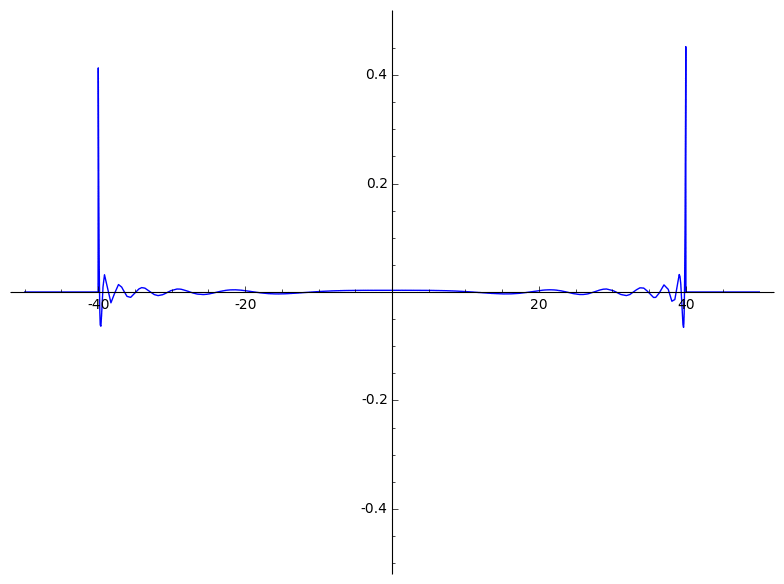
\includegraphics[width=\linewidth]{figures/propagator.png}
  \caption{Propagator $G(x-y)$ at $x-y = (40, \xi, 0, 0)$ and $m=1$.}
\end{figure}


\subsection{Propagator of the Free Field}

The propagator of a free scalar field is also a Green's function:
\begin{equation}
  \begin{split}
    \langle 0| \phi(x) \phi(y) |0\rangle =&\;
    \int \widetilde{dk} \int \widetilde{dk}' 
    \langle 0| a(\vec{k}) a^\dagger(\vec{k}') |0\rangle \; e^{i(kx-k'y)}
    \\    =&\;
    \int \frac{d^3\vec{k}}{(2\pi)^3}
    \frac{1}{2\omega} 
    e^{ik(x-y)}
    \\    =&\;
    \frac{1}{2} 
    \int \frac{d^3\vec{k}}{(2\pi)^3}
    \oint \frac{dk_0}{2\pi i}
    \frac{1}{k^2+m^2} 
    e^{ik(x-y)}
    \\    =&\;
    \frac{1}{2i} \Big(
    G_\text{Ret}(x-y) - G_\text{Adv}(x-y)
    \Big)
  \end{split}
\end{equation}
where the $\oint$-contour consists of two small circles around the two
poles, which is equals to the retarded Green's function contour minus
the advanced Green's function contour.


\subsection{Feynman Propagator}

There is a third choice of integration contour which turns out to be
the most useful for quantum field theory. of course we need the vacuum
expectation value of time-ordered products in quantum field theory, so
let us define
\begin{definition}[Feynman propagator]
  The Green's function $\Delta$ defined as 
  \begin{equation}
    \tfrac{1}{i} \Delta(x-y) = 
    \langle 0 | T \phi(x) \phi(y) |0\rangle
  \end{equation}
  is called the Feynman propagator.
\end{definition}
In terms of integration contour in the $k_0\in \C$ plane, this is the
path that goes below at $k_0=-\omega$ and above at $k_0=\omega$, see
\autoref{fig:feynman_propagator_path}. 
\begin{figure}
  \label{fig:feynman_propagator_path}
  \centering
  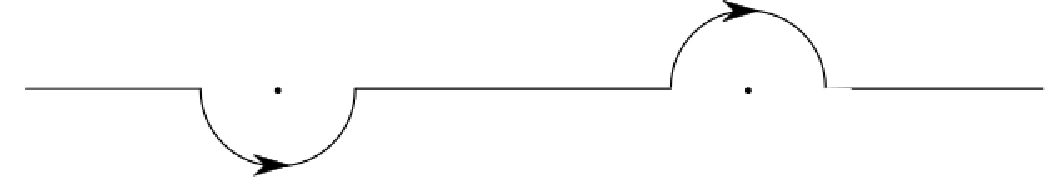
\includegraphics[width=\linewidth]{figures/FeynmanPropagatorPath.pdf}
  \caption{Feynman propagator integration contour in the $k_0\in \C$ plane.}
\end{figure}
Depending on whether $x$ is in the future or the past of $y$, this
contour selects the advanced or retarded Green's function. Finally, in
terms of an algebraic $i\epsilon$ prescription, the Feynman propagator
is
\begin{equation}
  \Delta(x-y) = 
  \lim_{\epsilon \to 0^+}
  \int
  \frac{d^4k}{(2\pi)^4}
  \frac{1}{k^2 + m^2 - i \epsilon}
  e^{ik(x-y)}
\end{equation}




\section{Week 3, Wednesday}






\newpage
\appendix

\section{test}



\bibliographystyle{utcaps} 
\renewcommand{\refname}{Bibliography}
\addcontentsline{toc}{section}{Bibliography} 
\bibliography{Main}


\end{document}


%%% Local Variables:
%%% eval: (TeX-PDF-mode 1)
%%% End:
